\section{Non-blocking Code}
\subsection{Aufgabenstellung}
Schreiben Sie ein Programm mit folgender Funktionalität:
\begin{itemize}%Aufzählung mit Numerierung
		\item Die 4 LEDs auf dem Board sollen mit unterschiedlichen Periodendauern blinken: 2*300ms, 2*500ms, 2*700ms und 2*1100ms blinken.
		\item Zu wie viel Prozent ist die CPU ausgelastet?
		\item Die Leuchtdauer der LEDs soll per Tastendruck einstellbar sein. Genau die Zeitdauer, während der ein zugeordneter Taster gedrückt ist, definiert den Sollwert für die halbe Periodendauer.
\end{itemize}
Hinweise zur Implementierung:
\begin{itemize}
	\item Wenden Sie das Konzept des kooperativen Multitaskings (non-blocking Code) an.
	\item Verwenden Sie getSystemTimeMillis().
\end{itemize}

\subsection{Lösung}
Bei der Implementierung der geforderten Funktionen wurde davon ausgegangen, dass die Funktionen zyklisch jede ms aufgerufen werden. Somit können die Funktionen losgelöst von Timern implementiert werden.\newline
Die Funktion zum zyklischen blinken der LED sind in Listening \ref{lst:blinkLed} dargestellt. Die Funktion zum messen der ToggleTime sind in Listening \ref{lst:measuretoggletimesw0} dargestellt. \newline
Die Auslastung der CPU liegt bei ca. 1\%. In Listening \ref{lst:mainnonblocking} ist die main Funktion dargestellt, diese stellt sicher, dass alle Funktionen zyklisch jede ms aufgerufen werden.

\begin{figure}[h]
	\centering
	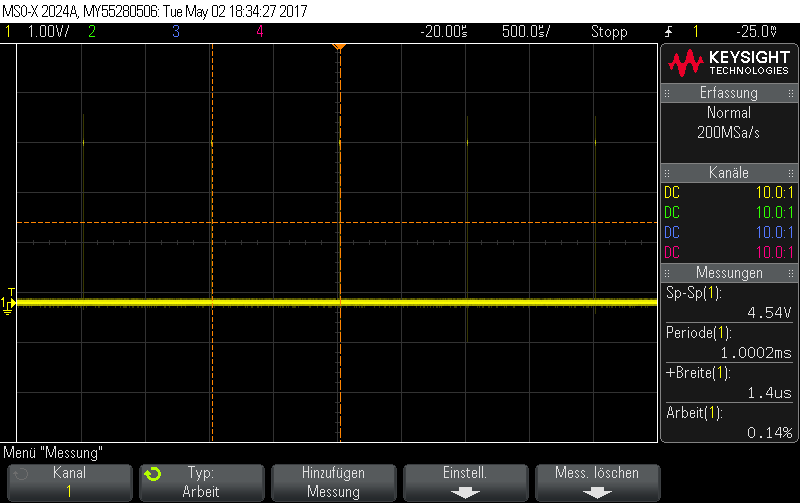
\includegraphics[width=0.7205\textwidth]{Images/scope_nonblockingcodepng}
	\caption[NonBlockingCode]{Auslastung der CPU}
	\label{image:nonblockingcode}
\end{figure}

\newpage
\begin{lstlisting}[frame=htrbl, caption={blinkLed0() Funktion}, label={lst:blinkLed}]
/** 
* @brief Toggle LED0 (RB_8) with toggle Time
* @param uint16_t ui16ToggleTime Toggle Time in Functions Calls
* @details Toggles RB_8 with the number of functions calls.
* @details Example: If Toggle Time is 20, you have to call the function 20 times to toggle RB_8
* @attention toggle pin has to be defined as digital output first
*/
void blinkLed0(uint16_t ui16ToggleTime)
{
  static uint16_t ui16Counter = 0;

  if(ui16ToggleTime == 0)
  {
    ui16Counter=0;
    digitalWrite(LED0,LOW);
    return;
  }
  else
    ui16Counter++;

  if(ui16Counter >= ui16ToggleTime)
  {
    ui16Counter=0;
    digitalToggle(LED0);
  }
}
\end{lstlisting}
\newpage
\begin{lstlisting}[frame=htrbl, caption={measureToggleTimeSW0() Funktion}, label={lst:measuretoggletimesw0}]
/** 
* @brief Measure hold Time from RG_12
* @returns uint16_t ui16HoldTime HoldTime is measured in function calls
* @details Measures Hold Time in Functions calls, if the Pin is not hold (high level) the functions retuns the last measured hold time
* @details Example: If the Pin is hold for 40ms you get the return value 40 when the function is called each ms, or the return value 20 when the function is called each 2ms
* @attention Pin has to be configured as input first, the functions is low active
*/
uint16_t measureToggleTimeSW0()
{
  static uint16_t ui16ToggleTime=0;
  static uint8_t  ui8MeasureMode=0;

  if(digitalRead(SW0)==LOW && (ui8MeasureMode==0))
  {
    ui16ToggleTime=0;
    ui8MeasureMode=1;
  }

  if(ui8MeasureMode==1)
  {
    ui16ToggleTime++;
  if(digitalRead(SW0)==HIGH)
    ui8MeasureMode=0;
  }

  return ui16ToggleTime;
}
\end{lstlisting}

\newpage
\begin{lstlisting}[frame=htrbl, caption={NonBlockingCode Main-Funktion}, label={lst:mainnonblocking}]
int main() {
	configOscillator();
	
	//set LED pinmodes
	pinMode(LED0,OUTPUT);
	pinMode(LED1,OUTPUT);
	pinMode(LED2,OUTPUT);
	pinMode(LED3,OUTPUT);
	
	//set switch pinmodes
	pinMode(SW0, INPUT_PULLUP);
	pinMode(SW1, INPUT_PULLUP);
	pinMode(SW2, INPUT_PULLUP);
	pinMode(SW3, INPUT_PULLUP);
	
	//config timer 1 for getSystemTimeMillis();)
	configSystemTimeMillis();
		
	/* Endless Loop */
	while(1){
		static uint32_t ui32Time= 0;
		
		blinkLed(LED0, measureToggleTimeSW(SW0));
		blinkLed(LED1, measureToggleTimeSW(SW1));
		blinkLed(LED2, measureToggleTimeSW(SW2));
		blinkLed(LED3, measureToggleTimeSW(SW3));
				
		ui32Time++; //increase ms counter
		while(getSystemTimeMillis() < ui32Time) //wait rest of 1ms
		{
			ClrWdt();   //clear watchdog timer
		}
	}//while
	return (EXIT_SUCCESS);  //never reached
} //main()
\end{lstlisting}

